\documentclass[12pt]{article}
\usepackage{fontspec}
\usepackage{fullpage}
\usepackage{hyperref}
\hypersetup{bookmarks=true,colorlinks=true,linkcolor=red,citecolor=blue,filecolor=magenta,urlcolor=cyan}
\usepackage{amsmath}
\usepackage{amssymb}
\usepackage{mathtools}
\usepackage{unicode-math}
\usepackage{tabu}
\usepackage{longtable}
\usepackage{booktabs}
\usepackage{caption}
\usepackage{graphics}
\usepackage{filecontents}
\usepackage[backend=bibtex]{biblatex}
\usepackage{url}
\newlist{symbDescription}{description}{1}
\setlist[symbDescription]{noitemsep, topsep=0pt, parsep=0pt, partopsep=0pt}
\setmathfont{Latin Modern Math}
\global\tabulinesep=1mm
\newcounter{assumpnum}
\newcommand{\atheassumpnum}{A\theassumpnum}
\newcounter{reqnum}
\newcommand{\rthereqnum}{R\thereqnum}
\newcounter{lcnum}
\newcommand{\lcthelcnum}{LC\thelcnum}
\newcounter{ucnum}
\newcommand{\uctheucnum}{UC\theucnum}
\bibliography{bibfile}
\title{Software Requirements Specification for GlassBR}
\author{Nikitha Krithnan and W. Spencer Smith}
\begin{document}
\maketitle
\tableofcontents
\newpage
\section{Reference Material}
\label{Sec:RefMat}
This section records information for easy reference.
\subsection{Table of Units}
\label{Sec:ToU}
The unit system used throughout is SI (Système International d'Unités). In addition to the basic units, several derived units are also used. For each unit, the table lists the symbol, a description and the SI name.
\begin{longtable*}{l l}
\toprule
Symbol & Description
\\
\midrule
kg & mass (kilogram)
\\
m & length (metre)
\\
N & force (newton)
\\
Pa & pressure (pascal)
\\
s & time (second)
\\
\bottomrule
\label{Table:ToU}
\end{longtable*}
\subsection{Table of Symbols}
\label{Sec:ToS}
The table that follows summarizes the symbols used in this document along with their units. The symbols are listed in alphabetical order.
\begin{longtabu}{l X[l] l}
\toprule
Symbol & Description & Units
\\
\midrule
$a$ & Plate length (long dimension) & m
\\
$AR$ & Aspect ratio & --
\\
${AR_{max}}$ & Maximum aspect ratio & --
\\
$B$ & Risk of failure & --
\\
$b$ & Plate width (short dimension) & m
\\
${d_{max}}$ & Maximum value for one of the dimensions of the glass plate & m
\\
${d_{min}}$ & Minimum value for one of the dimensions of the glass plate & m
\\
$E$ & Modulus of elasticity of glass & Pa
\\
$g$ & Glass type $g\in{}\{AN,FT,HS\}$ & --
\\
$GTF$ & Glass type factor & --
\\
$h$ & Minimum thickness & m
\\
$is\_safeLR$ & Variable that is assigned true when load resistance (capacity) is greater than load (demand) & --
\\
$is\_safePb$ & Variable that is assigned true when calculated probability is less than tolerable probability & --
\\
$J$ & Stress distribution factor (Function) & --
\\
${J_{tol}}$ & Stress distribution factor (Function) based on Pbtol & --
\\
$k$ & Surface flaw parameter & $\frac{\text{m}^{12}}{\text{N}^{7}}$
\\
$LDF$ & Load duration factor & --
\\
$LR$ & Load resistance & --
\\
$LSF$ & Load share factor & --
\\
$m$ & Surface flaw parameter & $\frac{\text{m}^{12}}{\text{N}^{7}}$
\\
$NFL$ & Non-factored load & --
\\
${P_{b}}$ & Probability of breakage & --
\\
${P_{btol}}$ & Tolerable probability of breakage & --
\\
$q$ & Applied load (demand) & Pa
\\
$\hat{q}$ & Dimensionless load & --
\\
${\hat{q}_{tol}}$ & Tolerable load & --
\\
$SD$ & Stand off distance & m
\\
${SD_{max}}$ & Maximum stand off distance permissible for input & m
\\
${SD_{min}}$ & Minimum stand off distance permissible for input & m
\\
${SD_{x}}$ & Stand off distance (x-component) & m
\\
${SD_{y}}$ & Stand off distance (y-component) & m
\\
${SD_{z}}$ & Stand off distance (z-component) & m
\\
$t$ & Nominal thickness $t\in{}\{2.5,2.7,3.0,4.0,5.0,6.0,8.0,10.0,12.0,16.0,19.0,22.0\}$ & mm
\\
${t_{d}}$ & Duration of load & s
\\
$TNT$ & TNT equivalent factor & --
\\
$w$ & Charge weight & kg
\\
${w_{max}}$ & Maximum permissible input charge weight & kg
\\
${w_{min}}$ & Minimum permissible input charge weight & kg
\\
${w_{TNT}}$ & Explosive mass in equivalent weight of TNT & kg
\\
\bottomrule
\label{Table:ToS}
\end{longtabu}
\subsection{Abbreviations and Acronyms}
\label{Sec:TAbbAcc}
\begin{longtable*}{l l}
\toprule
Abbreviation & Full Form
\\
\midrule
A & Assumption
\\
AN & Annealed
\\
AR & Aspect Ratio
\\
DD & Data Definition
\\
FT & Fully Tempered
\\
GS & Goal Statement
\\
GTF & Glass Type Factor
\\
HS & Heat Strengthened
\\
IG & Insulating Glass
\\
IM & Instance Model
\\
LC & Likely Change
\\
LG & Laminated Glass
\\
N/A & Not Applicable
\\
PS & Physical System Description
\\
R & Requirement
\\
SD & Stand Off Distance
\\
SRS & Software Requirements Specification
\\
T & Theoretical Model
\\
UC & Unlikely Change
\\
Uncert. & Typical Uncertainty
\\
\bottomrule
\label{Table:TAbbAcc}
\end{longtable*}
\section{Introduction}
\label{Sec:Intro}
Software is helpful to efficiently and correctly predict the blast risk involved with the glass slab. The blast under consideration is any kind of man-made explosion. The software, herein called GlassBR, aims to predict the blast risk involved with the glass slab using an intuitive interface.
The following section provides an overview of the Software Requirements Specification (SRS) for GlassBR. This section explains the purpose of this document, the scope of the system, the organization of the document, and the characteristics of the intended reader.
\subsection{Purpose of Document}
\label{Sec:DocPurpose}
The main purpose of this document is to predict whether a given glass slab is likely to resist a specified blast. The goals and theoretical models used in the GlassBR code are provided, with an emphasis on explicitly identifying assumptions and unambiguous definitions. This document is intended to be used as a reference to provide all information necessary to understand and verify the analysis. The SRS is abstract because the contents say what problem is being solved, but not how to solve it.
This document will be used as a starting point for subsequent development phases, including writing the design specification and the software verification and validation plan. The design document will show how the requirements are to be realized, including decisions on the numerical algorithms and programming environment. The verification and validation plan will show the steps that will be used to increase confidence in the software documentation and the implementation. Although the SRS fits in a series of documents that follow the so-called waterfall model, the actual development process is not constrained in any way. Even when the waterfall model is not followed, as Parnas and Clements point out \cite{parnasClements1986}, the most logical way to present the documentation is still to ``fake'' a rational design process.
\subsection{Scope of Requirements}
\label{Sec:ReqsScope}
The scope of the requirements includes getting all input parameters related to the glass slab and also the parameters related to blast type. Given the appropriate inputs, GlassBR predicts whether a glass slab is safe or not.
\subsection{Characteristics of Intended Reader}
\label{Sec:ReaderChars}
Reviewers of this documentation should have a strong knowledge in theory behind glass breakage and blast risk. The reviewers should also have an understanding of second year calculus, structural mechanics, and computer applications in civil engineering. In addition, reviewers should be familiar with the applicable standards for constructions using glass from {[}1-3{]} in Section~\ref{Sec:References}. The users of GlassBR can have a lower level of expertise, as explained in Section~\ref{Sec:UserChars}.
\subsection{Organization of Document}
\label{Sec:DocOrg}
The organization of this document follows the template for an SRS for scientific computing software proposed by \cite{koothoor2013} and \cite{smithLai2005}, with some aspects taken from Volere template 16 \cite{rbrtsn2012}. The presentation follows the standard pattern of presenting goals, theories, definitions, and assumptions. For readers that would like a more bottom up approach, they can start reading the data definitions in Section~\ref{Sec:DDs} and trace back to find any additional information they require.
The goal statements are refined to the theoretical models, and the theoretical models to the instance models. The data definitions are used to support the definitions of the different models.
\section{Stakeholders}
\label{Sec:Stakeholder}
This section describes the stakeholders: the people who have an interest in the product.
\subsection{The Client}
\label{Sec:Client}
The client for GlassBR is a company named Entuitive. It is developed by Dr. Manuel Campidelli. The client has the final say on acceptance of the product.
\subsection{The Customer}
\label{Sec:Customer}
The customers are the end user of GlassBR.
\section{General System Description}
\label{Sec:GenSysDesc}
This section provides general information about the system including identifying the interfaces between the system and its environment (system context), describing the user characteristics and listing the system constraints.
\subsection{System Context}
\label{Sec:SysContext}
Figure~\ref{Figure:sysCtxDiag} shows the system context. A circle represents an external entity outside the software, the user in this case. A rectangle represents the software system itself (GlassBR). Arrows are used to show the data flow between the system and its environment.
\begin{figure}
\begin{center}
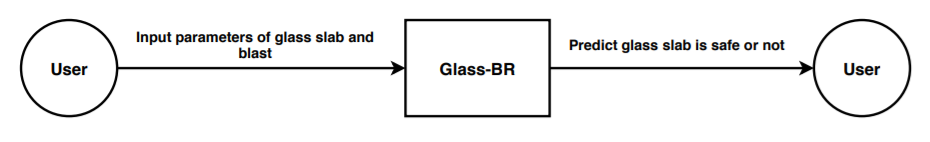
\includegraphics[width=\textwidth]{../../../datafiles/GlassBR/SystemContextFigure.png}
\caption{System Context}
\label{Figure:sysCtxDiag}
\end{center}
\end{figure}
The interaction between the product and the user is through a user interface. The responsibilities of the user and the system are as follows:
\begin{itemize}
\item{User Responsibilities}
\begin{itemize}
\item{Provide the input data related to the glass slab and blast}
\item{type ensuring no errors in the data entry}
\item{Ensure that consistent units are used for input variables}
\item{Ensure required software assumptions (FIXME REF) are appropriate for any particular problem input to the software}
\end{itemize}
\item{GlassBR Responsibilities}
\begin{itemize}
\item{Detect data type mismatch, such as a string of characters}
\item{input instead of a floating point number}
\item{Determine if the inputs satisfy the required physical and software constraints}
\item{Predict whether the glass slab is safe or not.}
\end{itemize}
\end{itemize}
\subsection{User Characteristics}
\label{Sec:UserChars}
\begin{itemize}
\item{The end user of GlassBR is expected to have completed at least the equivalent of the second year of an undergraduate degree in civil engineering or structural engineering.}
\item{The end user is expected to have an understanding of theory behind glass breakage and blast risk.}
\item{The end user is expected to have basic computer literacy to handle the software.}
\end{itemize}
\subsection{System Constraints}
\label{Sec:SysConstraints}
There are no system constraints.
\section{Scope of the Project}
\label{Sec:ProjScope}
This section presents the scope of the project. It describes the expected use of GlassBR as well as the inputs and outputs of each action. The use cases are input and output, which defines the action of getting the input and displaying the output.
\subsection{Product Use Case Table}
\label{Sec:UseCaseTable}
\begin{longtabu}{l X[l]}
\toprule
Actor & Input and Output
\\
\midrule
User & Characteristics of the glass slab and of the blast. Details in Section~\ref{Sec:IndividualProdUC}
\\
GlassBR & Whether or not the glass slab is safe for the calculated load and supporting calculated values
\\
\bottomrule
\caption{Use Case Table}
\label{Table:useCaseTable}
\end{longtabu}
\subsection{Individual Product Use Cases}
\label{Sec:IndividualProdUC}
The user provides the inputs to GlassBR for use within the analysis. There are two main classes of inputs: glass geometry and blast type. The glass geometry based inputs include the glass type and dimensions of the glass plane. The blast type input includes parameters like weight of charge, TNT equivalent factor, and stand off distance from the point of explosion. These parameters describe charge weight and stand off blast. Another input the user gives is the tolerable value of probability of breakage. GlassBR outputs if the glass slab will be safe by comparing whether capacity is greater than demand. Capacity is the load resistance calculated and demand is the requirement which is the 3 second duration equivalent pressure. The second condition is to check whether the calculated probability (${P_{b}}$) is less than the tolerable probability (${P_{btol}}$) which is obtained from the user as an input. If both conditions return true, then it's shown that the glass slab is safe to use, else if both return false, then the glass slab is considered unsafe. All the supporting calculated values are also displayed as output.
\section{Specific System Description}
\label{Sec:SpecSystDesc}
This section first presents the problem description, which gives a high-level view of the problem to be solved. This is followed by the solution characteristics specification, which presents the assumptions, theories, and definitions that are used.
\subsection{Problem Description}
\label{Sec:ProbDesc}
A system is needed to efficiently and correctly predict the blast risk involved with the glass. GlassBR is a computer program developed to interpret the inputs to give out the outputs which predict whether the glass slab can withstand the blast under the conditions.
\subsubsection{Terminology and Definitions}
\label{Sec:TermDefs}
This subsection provides a list of terms that are used in the subsequent sections and their meaning, with the purpose of reducing ambiguity and making it easier to correctly understand the requirements. All of the terms are extracted from {[}1{]} in Section~\ref{Sec:References}.
\begin{enumerate}
\item{Glass breakage - The fracture or breakage of any lite or ply in monolithic, laminated, or insulating glass.}
\item{Lateral - Perpendicular to the glass surface.}
\item{Lite - Pieces of glass that are cut, prepared, and used to create the window or door.}
\item{Specifying authority - The design professional responsible for interpreting applicable regulations of authorities having jurisdiction and considering appropriate site specific factors to determine the appropriate values used to calculate the specified design load, and furnishing other information required to perform this practice.}
\item{Blast resistant glazing - Glazing that provides protection against air blast pressure generated by explosions.}
\item{Equivalent TNT charge mass - Mass of TNT placed on the ground in a hemisphere that represents the design explosive threat.}
\item{Glass Type:}
\begin{itemize}
\item{Annealed (AN) - A flat, monolithic, glass lite which has uniform thickness where the residual surface stresses are almost zero, as defined in [3].}
\item{Fully tempered (FT) - A flat, monolithic, glass lite of uniform thickness that has been subjected to a special heat treatment process where the residual surface compression is not less than 69 MPa (10 000 psi) or the edge compression not less than 67 MPa (9700 psi), as defined in [2].}
\item{Heat strengthened (HS) - A flat, monolithic, glass lite of uniform thickness that has been subjected to a special heat treatment process where the residual surface compression is not less than 24 MPa (3500psi) or greater than 52 MPa (7500 psi), as defined in [2].}
\end{itemize}
\item{Load- A uniformly distributed lateral pressure.}
\begin{itemize}
\item{Load resistance (LR) - The uniform lateral load that a glass construction can sustain based upon a given probability of breakage and load duration as defined in [1 (pg. 1, 53)], following A2 and A1 respectively.}
\item{Non-factored load (NFL) - Three second duration uniform load associated with a probability of breakage less than or equal to 8 lites per 1000 for monolithic AN glass.}
\item{Glass weight load - The dead load component of the glass weight.}
\item{Short duration load - Any load lasting 3 seconds or less.}
\item{Specified design load - The magnitude in Pa (psf), type (for example, wind or snow) and duration of the load given by the specifying authority.}
\item{Long duration load - Any load lasting approximately 30 days.}
\end{itemize}
\item{Stand off distance (SD) - The distance from the glazing surface to the centroid of a hemispherical high explosive charge. It is represented by the coordinates (${SD_{x}}$, ${SD_{y}}$, ${SD_{z}}$).}
\item{Load share factor (LSF) - A multiplying factor derived from the load sharing between the double glazing, of equal or different thicknesses and types (including the layered behaviour of LG under long duration loads), in a sealed IG unit.}
\item{Glass type factor (GTF) - A multiplying factor for adjusting the LR of different glass type, that is, AN, FT, or HS, in monolithic glass, LG (Laminated Glass), or IG (Insulating Glass) constructions.}
\item{Aspect ratio (AR) - The ratio of the long dimension of the glass to the short dimension of the glass. For glass supported on four sides, the aspect ratio is always equal to or greater than 1.0. For glass supported on three sides, the ratio of the length of one of the supported edges perpendicular to the free edge, to the length of the free edge, is equal to or greater than 0.5.}
\item{Probability of breakage (${P_{b}}$) - The fraction of glass lites or plies that would break at the first occurrence of a specified load and duration, typically expressed in lites per 1000 [3].}
\end{enumerate}
\subsubsection{Physical System Description}
\label{Sec:PhysSyst}
The physical system of GlassBR, as shown in Figure~\ref{Figure:physSystImage}, includes the following elements:
\begin{itemize}
\item[PS1:]The glass slab.
\item[PS2:]The point of explosion. Where the bomb, or any kind of man-made explosion, is located. The stand off distance is the distance between the point of explosion and the glass.
\end{itemize}
\begin{figure}
\begin{center}
\includegraphics[width=0.3\textwidth]{../../../datafiles/GlassBR/physicalsystimage.png}
\caption{The physical system}
\label{Figure:physSystImage}
\end{center}
\end{figure}
\subsubsection{Goal Statements}
\label{Sec:GoalStmt}
Given the dimensions of the glass plane, glass type, the characteristics of the explosion, and the tolerable probability of breakage, the goal statements are:
\begin{itemize}
\item[GS1:]Analyze and predict whether the glass slab under consideration will be able to withstand the explosion of a certain degree which is calculated based on user input.
\end{itemize}
\subsection{Solution Characteristics Specification}
\label{Sec:SolCharSpec}
The instance models that govern GlassBR are presented in Section~\ref{Sec:IMs}. The information to understand the meaning of the instance models and their derivation is also presented, so that the instance models can be verified.
\subsubsection{Assumptions}
\label{Sec:Assumps}
This section simplifies the original problem and helps in developing the theoretical model by filling in the missing information for the physical system. The numbers given in the square brackets refer to the Theoretical Models {[}Section~\ref{Sec:TMs}{]}, General Definitions {[}Section~\ref{Sec:GDs}{]}, Data Definitions {[}Section~\ref{Sec:DDs}{]}, Instance Models {[}Section~\ref{Sec:IMs}{]}, Likely Changes {[}Section~\ref{Sec:LCs}{]}, or Unlikely Changes {[}Section~\ref{Sec:UCs}{]}, in which the respective assumption is used.
\begin{description}
\item[\refstepcounter{assumpnum}\atheassumpnum\label{A:glassTy}:]The standard E1300-09a for calculation applies only to monolithic, laminated, or insulating glass constructions of rectangular shape with continuous lateral support along one, two, three, or four edges. This practice assumes that: (1) the supported glass edges for two, three and four-sided support conditions are simply supported and free to slip in plane; (2) glass supported on two sides acts as a simply supported beam; and (3) glass supported on one side acts as a cantilever.
\end{description}
\begin{description}
\item[\refstepcounter{assumpnum}\atheassumpnum\label{A:glassCondition}:]Following \cite{astm2009} (pg. 1), this practice does not apply to any form of wired, patterned, etched, sandblasted, drilled, notched, or grooved glass with surface and edge treatments that alter the glass strength.
\end{description}
\begin{description}
\item[\refstepcounter{assumpnum}\atheassumpnum\label{A:explainScenario}:]This system only considers the external explosion scenario for its calculations.
\end{description}
\begin{description}
\item[\refstepcounter{assumpnum}\atheassumpnum\label{A:standardValues}:]The values provided in Section~\ref{Sec:AuxConstants} are assumed for the duration of load (${t_{d}}$), and the material properties of $m$, $k$, and $E$. [IM1, DD3, DD5, DD7, DD9]
\end{description}
\begin{description}
\item[\refstepcounter{assumpnum}\atheassumpnum\label{A:glassLite}:]Glass under consideration is assumed to be a single lite; hence, the value of LSF is equal to 1 for all calculations in GlassBR. [IM2, DD7]
\end{description}
\begin{description}
\item[\refstepcounter{assumpnum}\atheassumpnum\label{A:boundaryConditions}:]Boundary conditions for the glass slab are assumed to be 4-sided support for calculations. [IM1]
\end{description}
\begin{description}
\item[\refstepcounter{assumpnum}\atheassumpnum\label{A:responseType}:]The response type considered in GlassBR is flexural. [IM1]
\end{description}
\begin{description}
\item[\refstepcounter{assumpnum}\atheassumpnum\label{A:ldfConstant}:]With reference to A\ref{A:standardValues}, the value of load duration factor ($LDF$) is a constant in GlassBR. [DD3]
\end{description}
\subsubsection{Theoretical Models}
\label{Sec:TMs}
This section focuses on the general equations and laws that GlassBR is based on.
~\newline
\noindent \begin{minipage}{\textwidth}
\begin{tabular}{p{0.2\textwidth} p{0.73\textwidth}}
\toprule \textbf{Refname} & \textbf{T:isSafePb}
\phantomsection 
\label{T:isSafePb}
\\ \midrule \\
Label & Safety Req-Pb
\\ \midrule \\
Equation & \begin{dmath}
           is\_safePb={P_{b}}<{P_{btol}}
           \end{dmath}
\\ \midrule \\
Description & \begin{symbDescription}
              \item{$is\_safePb$ is the variable that is assigned true when calculated probability is less than tolerable probability (Unitless)}
              \item{${P_{b}}$ is the probability of breakage (Unitless)}
              \item{${P_{btol}}$ is the tolerable probability of breakage (Unitless)}
              \end{symbDescription}
\\ \midrule \\
Notes & If $is\_safePb$, the glass is considered safe. $is\_safePb$ and $is\_safeLR$ (from \hyperref[T:isSafeLR]{Definition~T:isSafeLR}) are either both True or both False. ${P_{b}}$ is the probability of breakage, as calculated in \hyperref[IM:probOfBr]{Definition~IM:probOfBr}. ${P_{btol}}$ is the tolerable probability of breakage entered by the user.
\\ \midrule \\
Source & FIXME: This needs to be filled in
\\ \midrule \\
RefBy & FIXME: This needs to be filled in
\\ \bottomrule \end{tabular}
\end{minipage}\\
~\newline
\noindent \begin{minipage}{\textwidth}
\begin{tabular}{p{0.2\textwidth} p{0.73\textwidth}}
\toprule \textbf{Refname} & \textbf{T:isSafeLR}
\phantomsection 
\label{T:isSafeLR}
\\ \midrule \\
Label & Safety Req-LR
\\ \midrule \\
Equation & \begin{dmath}
           is\_safeLR=LR>q
           \end{dmath}
\\ \midrule \\
Description & \begin{symbDescription}
              \item{$is\_safeLR$ is the variable that is assigned true when load resistance (capacity) is greater than load (demand) (Unitless)}
              \item{$LR$ is the load resistance (Unitless)}
              \item{$q$ is the applied load (demand) (Pa)}
              \end{symbDescription}
\\ \midrule \\
Notes & If $is\_safeLR$, the glass is considered safe. $is\_safePb$ (from \hyperref[T:isSafePb]{Definition~T:isSafePb}) and $is\_safeLR$ are either both True or both False. LR is the load resistance (also called capacity), as defined in \hyperref[IM:calOfCap]{Definition~IM:calOfCap}. $q$ (also referred as the Demand) is the 3 second duration equivalent pressure, as defined in \hyperref[IM:calOfDemand]{Definition~IM:calOfDemand}.
\\ \midrule \\
Source & FIXME: This needs to be filled in
\\ \midrule \\
RefBy & FIXME: This needs to be filled in
\\ \bottomrule \end{tabular}
\end{minipage}\\
\subsubsection{General Definitions}
\label{Sec:GDs}
There are no general definitions.
\subsubsection{Data Definitions}
\label{Sec:DDs}
This section collects and defines all the data needed to build the instance models.
~\newline
\noindent \begin{minipage}{\textwidth}
\begin{tabular}{p{0.2\textwidth} p{0.73\textwidth}}
\toprule \textbf{Refname} & \textbf{DD:risk.fun}
\phantomsection 
\label{DD:risk.fun}
\\ \midrule \\
Label & Risk of failure
\\ \midrule \\
Symbol & $B$
\\ \midrule \\
Units & Unitless
\\ \midrule \\
Equation & \begin{dmath}
           B=\frac{k}{\left(a b\right)^{m-1}} \left(E h^{2}\right)^{m} LDF e^{J}
           \end{dmath}
\\ \midrule \\
Description & \begin{symbDescription}
              \item{$B$ is the risk of failure (Unitless)}
              \item{$k$ is the surface flaw parameter ($\frac{\text{m}^{12}}{\text{N}^{7}}$)}
              \item{$a$ is the plate length (long dimension) (m)}
              \item{$b$ is the plate width (short dimension) (m)}
              \item{$m$ is the surface flaw parameter ($\frac{\text{m}^{12}}{\text{N}^{7}}$)}
              \item{$E$ is the modulus of elasticity of glass (Pa)}
              \item{$h$ is the minimum thickness (m)}
              \item{$LDF$ is the load duration factor (Unitless)}
              \item{$J$ is the stress distribution factor (Function) (Unitless)}
              \end{symbDescription}
\\ \midrule \\
Notes & $a$, $b$ are dimensions of the plate, where ($a\geq{}b$).
        $h$ is the minimum thickness, which is based on the nominal thicknesses as shown in DD2.
        $LDF$ is the load duration factor as defined by DD3.
        $J$ is the stress distribution factor (Function) , as defined in DD4.
\\ \midrule \\
Source & [1] [4, Eq. 4-5] [5, Eq. 14]
\\ \midrule \\
RefBy & FIXME: This needs to be filled in
\\ \bottomrule \end{tabular}
\end{minipage}\\
~\newline
\noindent \begin{minipage}{\textwidth}
\begin{tabular}{p{0.2\textwidth} p{0.73\textwidth}}
\toprule \textbf{Refname} & \textbf{DD:min.thick}
\phantomsection 
\label{DD:min.thick}
\\ \midrule \\
Label & Minimum thickness
\\ \midrule \\
Symbol & $h$
\\ \midrule \\
Units & m
\\ \midrule \\
Equation & \begin{dmath}
           h=\frac{1}{1000} \begin{cases}
2.16, & t=2.5\\
2.59, & t=2.7\\
2.92, & t=3.0\\
3.78, & t=4.0\\
4.57, & t=5.0\\
5.56, & t=6.0\\
7.42, & t=8.0\\
9.02, & t=10.0\\
11.91, & t=12.0\\
15.09, & t=16.0\\
18.26, & t=19.0\\
21.44, & t=22.0
\end{cases}
           \end{dmath}
\\ \midrule \\
Description & \begin{symbDescription}
              \item{$h$ is the minimum thickness (m)}
              \item{$t$ is the nominal thickness $t\in{}\{2.5,2.7,3.0,4.0,5.0,6.0,8.0,10.0,12.0,16.0,19.0,22.0\}$ (mm)}
              \end{symbDescription}
\\ \midrule \\
Notes & $t$ is a function that maps from the nominal thickness ($h$) to the minimum thickness.
\\ \midrule \\
Source & 
\\ \midrule \\
RefBy & FIXME: This needs to be filled in
\\ \bottomrule \end{tabular}
\end{minipage}\\
~\newline
\noindent \begin{minipage}{\textwidth}
\begin{tabular}{p{0.2\textwidth} p{0.73\textwidth}}
\toprule \textbf{Refname} & \textbf{DD:loadDurFactor}
\phantomsection 
\label{DD:loadDurFactor}
\\ \midrule \\
Label & Load duration factor
\\ \midrule \\
Symbol & $LDF$
\\ \midrule \\
Units & Unitless
\\ \midrule \\
Equation & \begin{dmath}
           LDF=\left(\frac{{t_{d}}}{60}\right)^{\frac{m}{16}}
           \end{dmath}
\\ \midrule \\
Description & \begin{symbDescription}
              \item{$LDF$ is the load duration factor (Unitless)}
              \item{${t_{d}}$ is the duration of load (s)}
              \item{$m$ is the surface flaw parameter ($\frac{\text{m}^{12}}{\text{N}^{7}}$)}
              \end{symbDescription}
\\ \midrule \\
Source & 
\\ \midrule \\
RefBy & FIXME: This needs to be filled in
\\ \bottomrule \end{tabular}
\end{minipage}\\
~\newline
\noindent \begin{minipage}{\textwidth}
\begin{tabular}{p{0.2\textwidth} p{0.73\textwidth}}
\toprule \textbf{Refname} & \textbf{DD:stressDistFac}
\phantomsection 
\label{DD:stressDistFac}
\\ \midrule \\
Label & Stress distribution factor (Function)
\\ \midrule \\
Symbol & $J$
\\ \midrule \\
Units & Unitless
\\ \midrule \\
Equation & \begin{dmath}
           J=J\left(\hat{q},AR\right)
           \end{dmath}
\\ \midrule \\
Description & \begin{symbDescription}
              \item{$J$ is the stress distribution factor (Function) (Unitless)}
              \item{$J$ is the stress distribution factor (Function) (Unitless)}
              \item{$\hat{q}$ is the dimensionless load (Unitless)}
              \item{$AR$ is the aspect ratio (Unitless)}
              \end{symbDescription}
\\ \midrule \\
Notes & $J$ is the stress distribution factor (Function), which is obtained by interpolating from data shown in Figure 7.
        $\hat{q}$ is the dimensionless load defined in DD7.
        $AR$ is the aspect ratio defined in DD11.
\\ \midrule \\
Source & 
\\ \midrule \\
RefBy & FIXME: This needs to be filled in
\\ \bottomrule \end{tabular}
\end{minipage}\\
~\newline
\noindent \begin{minipage}{\textwidth}
\begin{tabular}{p{0.2\textwidth} p{0.73\textwidth}}
\toprule \textbf{Refname} & \textbf{DD:nFL}
\phantomsection 
\label{DD:nFL}
\\ \midrule \\
Label & Non-factored load
\\ \midrule \\
Symbol & $NFL$
\\ \midrule \\
Units & Unitless
\\ \midrule \\
Equation & \begin{dmath}
           NFL=\frac{{\hat{q}_{tol}} E h^{4}}{\left(a b\right)^{2}}
           \end{dmath}
\\ \midrule \\
Description & \begin{symbDescription}
              \item{$NFL$ is the non-factored load (Unitless)}
              \item{${\hat{q}_{tol}}$ is the tolerable load (Unitless)}
              \item{$E$ is the modulus of elasticity of glass (Pa)}
              \item{$h$ is the minimum thickness (m)}
              \item{$a$ is the plate length (long dimension) (m)}
              \item{$b$ is the plate width (short dimension) (m)}
              \end{symbDescription}
\\ \midrule \\
Notes & $a$, $b$ are dimensions of the plate, where ($a\geq{}b$).
        $h$ is the minimum thickness, which is based on the nominal thicknesses as shown in DD2.
        ${\hat{q}_{tol}}$ is the tolerable load defined in DD8.
\\ \midrule \\
Source & 
\\ \midrule \\
RefBy & FIXME: This needs to be filled in
\\ \bottomrule \end{tabular}
\end{minipage}\\
~\newline
\noindent \begin{minipage}{\textwidth}
\begin{tabular}{p{0.2\textwidth} p{0.73\textwidth}}
\toprule \textbf{Refname} & \textbf{DD:gTF}
\phantomsection 
\label{DD:gTF}
\\ \midrule \\
Label & Glass type factor
\\ \midrule \\
Symbol & $GTF$
\\ \midrule \\
Units & Unitless
\\ \midrule \\
Equation & \begin{dmath}
           GTF=\begin{cases}
1, & g=AN\\
4, & g=FT\\
2, & g=HS
\end{cases}
           \end{dmath}
\\ \midrule \\
Description & \begin{symbDescription}
              \item{$GTF$ is the glass type factor (Unitless)}
              \item{$g$ is the glass type $g\in{}\{AN,FT,HS\}$ (Unitless)}
              \end{symbDescription}
\\ \midrule \\
Notes & AN is annealed glass
        FT is fully tempered glass
        HS is heat strengthened glass
\\ \midrule \\
Source & 
\\ \midrule \\
RefBy & FIXME: This needs to be filled in
\\ \bottomrule \end{tabular}
\end{minipage}\\
~\newline
\noindent \begin{minipage}{\textwidth}
\begin{tabular}{p{0.2\textwidth} p{0.73\textwidth}}
\toprule \textbf{Refname} & \textbf{DD:dimlessLoad}
\phantomsection 
\label{DD:dimlessLoad}
\\ \midrule \\
Label & Dimensionless load
\\ \midrule \\
Symbol & $\hat{q}$
\\ \midrule \\
Units & Unitless
\\ \midrule \\
Equation & \begin{dmath}
           \hat{q}=\frac{q \left(a b\right)^{2}}{E h^{4} GTF}
           \end{dmath}
\\ \midrule \\
Description & \begin{symbDescription}
              \item{$\hat{q}$ is the dimensionless load (Unitless)}
              \item{$q$ is the applied load (demand) (Pa)}
              \item{$a$ is the plate length (long dimension) (m)}
              \item{$b$ is the plate width (short dimension) (m)}
              \item{$E$ is the modulus of elasticity of glass (Pa)}
              \item{$h$ is the minimum thickness (m)}
              \item{$GTF$ is the glass type factor (Unitless)}
              \end{symbDescription}
\\ \midrule \\
Notes & $q$ is the 3 second equivalent pressure, as given in IM3.
        $a$, $b$ are dimensions of the plate, where ($a\geq{}b$).
        $h$ is the minimum thickness, which is based on the nominal thicknesses as shown in DD2.
        $GTF$ is the glass type factor, as given by DD6.
        $\hat{q}$ is calculated with reference to A\ref{A:glassLite}.
\\ \midrule \\
Source & [5, Eq. 7]
\\ \midrule \\
RefBy & FIXME: This needs to be filled in
\\ \bottomrule \end{tabular}
\end{minipage}\\
~\newline
\noindent \begin{minipage}{\textwidth}
\begin{tabular}{p{0.2\textwidth} p{0.73\textwidth}}
\toprule \textbf{Refname} & \textbf{DD:tolLoad}
\phantomsection 
\label{DD:tolLoad}
\\ \midrule \\
Label & Tolerable load
\\ \midrule \\
Symbol & ${\hat{q}_{tol}}$
\\ \midrule \\
Units & Unitless
\\ \midrule \\
Equation & \begin{dmath}
           {\hat{q}_{tol}}={\hat{q}_{tol}}\left({J_{tol}},\frac{a}{b}\right)
           \end{dmath}
\\ \midrule \\
Description & \begin{symbDescription}
              \item{${\hat{q}_{tol}}$ is the tolerable load (Unitless)}
              \item{${\hat{q}_{tol}}$ is the tolerable load (Unitless)}
              \item{${J_{tol}}$ is the stress distribution factor (Function) based on Pbtol (Unitless)}
              \item{$a$ is the plate length (long dimension) (m)}
              \item{$b$ is the plate width (short dimension) (m)}
              \end{symbDescription}
\\ \midrule \\
Notes & ${\hat{q}_{tol}}$ is the tolerable load which is obtained from Figure 7 using ${J_{tol}}$ and aspect ratio as parameters using interpolation. Calculations of ${J_{tol}}$ and $AR$ are defined in DD9 and DD11, respectively.
\\ \midrule \\
Source & 
\\ \midrule \\
RefBy & FIXME: This needs to be filled in
\\ \bottomrule \end{tabular}
\end{minipage}\\
~\newline
\noindent \begin{minipage}{\textwidth}
\begin{tabular}{p{0.2\textwidth} p{0.73\textwidth}}
\toprule \textbf{Refname} & \textbf{DD:sdf.tol}
\phantomsection 
\label{DD:sdf.tol}
\\ \midrule \\
Label & Stress distribution factor (Function) based on Pbtol
\\ \midrule \\
Symbol & ${J_{tol}}$
\\ \midrule \\
Units & Unitless
\\ \midrule \\
Equation & \begin{dmath}
           {J_{tol}}=\ln\left(\ln\left(\frac{1}{1-{P_{btol}}}\right) \frac{\left(a b\right)^{m-1}}{k \left(E h^{2}\right)^{m} LDF}\right)
           \end{dmath}
\\ \midrule \\
Description & \begin{symbDescription}
              \item{${J_{tol}}$ is the stress distribution factor (Function) based on Pbtol (Unitless)}
              \item{${P_{btol}}$ is the tolerable probability of breakage (Unitless)}
              \item{$a$ is the plate length (long dimension) (m)}
              \item{$b$ is the plate width (short dimension) (m)}
              \item{$m$ is the surface flaw parameter ($\frac{\text{m}^{12}}{\text{N}^{7}}$)}
              \item{$k$ is the surface flaw parameter ($\frac{\text{m}^{12}}{\text{N}^{7}}$)}
              \item{$E$ is the modulus of elasticity of glass (Pa)}
              \item{$h$ is the minimum thickness (m)}
              \item{$LDF$ is the load duration factor (Unitless)}
              \end{symbDescription}
\\ \midrule \\
Notes & ${J_{tol}}$  is calculated with reference to  ${P_{btol}}$.
        $a$, $b$ are dimensions of the plate, where ($a\geq{}b$).
        $h$ is the minimum thickness, which is based on the nominal thicknesses as shown in DD2.
        $LDF$ is the load duration factor as defined by DD3.
        ${P_{btol}}$ is the tolerable probability entered by the user.
\\ \midrule \\
Source & 
\\ \midrule \\
RefBy & FIXME: This needs to be filled in
\\ \bottomrule \end{tabular}
\end{minipage}\\
~\newline
\noindent \begin{minipage}{\textwidth}
\begin{tabular}{p{0.2\textwidth} p{0.73\textwidth}}
\toprule \textbf{Refname} & \textbf{DD:standOffDist}
\phantomsection 
\label{DD:standOffDist}
\\ \midrule \\
Label & Stand off distance
\\ \midrule \\
Symbol & $SD$
\\ \midrule \\
Units & m
\\ \midrule \\
Equation & \begin{dmath}
           SD=\sqrt{{SD_{x}}^{2}+{SD_{y}}^{2}+{SD_{z}}^{2}}
           \end{dmath}
\\ \midrule \\
Description & \begin{symbDescription}
              \item{$SD$ is the stand off distance (m)}
              \item{${SD_{x}}$ is the stand off distance (x-component) (m)}
              \item{${SD_{y}}$ is the stand off distance (y-component) (m)}
              \item{${SD_{z}}$ is the stand off distance (z-component) (m)}
              \end{symbDescription}
\\ \midrule \\
Source & 
\\ \midrule \\
RefBy & FIXME: This needs to be filled in
\\ \bottomrule \end{tabular}
\end{minipage}\\
~\newline
\noindent \begin{minipage}{\textwidth}
\begin{tabular}{p{0.2\textwidth} p{0.73\textwidth}}
\toprule \textbf{Refname} & \textbf{DD:aspect.ratio}
\phantomsection 
\label{DD:aspect.ratio}
\\ \midrule \\
Label & Aspect ratio
\\ \midrule \\
Symbol & $AR$
\\ \midrule \\
Units & Unitless
\\ \midrule \\
Equation & \begin{dmath}
           AR=\frac{a}{b}
           \end{dmath}
\\ \midrule \\
Description & \begin{symbDescription}
              \item{$AR$ is the aspect ratio (Unitless)}
              \item{$a$ is the plate length (long dimension) (m)}
              \item{$b$ is the plate width (short dimension) (m)}
              \end{symbDescription}
\\ \midrule \\
Notes & $a$, $b$ are dimensions of the plate, where ($a\geq{}b$).
\\ \midrule \\
Source & 
\\ \midrule \\
RefBy & FIXME: This needs to be filled in
\\ \bottomrule \end{tabular}
\end{minipage}\\
\subsubsection{Instance Models}
\label{Sec:IMs}
This section transforms the problem defined in Section~\ref{Sec:ProbDesc} into one which is expressed in mathematical terms. It uses concrete symbols defined in Section~\ref{Sec:DDs} to replace the abstract symbols in the models identified in Section~\ref{Sec:TMs} and Section~\ref{Sec:GDs}.
~\newline
\noindent \begin{minipage}{\textwidth}
\begin{tabular}{p{0.2\textwidth} p{0.73\textwidth}}
\toprule \textbf{Refname} & \textbf{IM:probOfBr}
\phantomsection 
\label{IM:probOfBr}
\\ \midrule \\
Label & Probability of Glass Breakage
\\ \midrule \\
Input & $B$
\\ \midrule \\
Output & ${P_{b}}$
\\ \midrule \\
Input Constraints & \begin{dmath}
                    B>0
                    \end{dmath}
\\ \midrule \\
Output Constraints & \begin{dmath}
                     {P_{b}}>0
                     \end{dmath}
\\ \midrule \\
Equation & \begin{dmath}
           {P_{b}}=1-e^{-B}
           \end{dmath}
\\ \midrule \\
Description & \begin{symbDescription}
              \item{${P_{b}}$ is the probability of breakage (Unitless)}
              \item{$B$ is the risk of failure (Unitless)}
              \end{symbDescription}
\\ \midrule \\
Source & [1] [4]
\\ \midrule \\
RefBy & FIXME: This needs to be filled in
\\ \bottomrule \end{tabular}
\end{minipage}\\
~\newline
\noindent \begin{minipage}{\textwidth}
\begin{tabular}{p{0.2\textwidth} p{0.73\textwidth}}
\toprule \textbf{Refname} & \textbf{IM:calOfCap}
\phantomsection 
\label{IM:calOfCap}
\\ \midrule \\
Label & Calculation of Capacity(LR)
\\ \midrule \\
Input & $NFL$, $GTF$, $LSF$
\\ \midrule \\
Output & $LR$
\\ \midrule \\
Input Constraints & \begin{dmath}
                    NFL>0
                    \end{dmath}
                    \begin{dmath}
                    GTF>0
                    \end{dmath}
                    \begin{dmath}
                    LSF>0
                    \end{dmath}
\\ \midrule \\
Output Constraints & 
\\ \midrule \\
Equation & \begin{dmath}
           LR=NFL GTF LSF
           \end{dmath}
\\ \midrule \\
Description & \begin{symbDescription}
              \item{$LR$ is the load resistance (Unitless)}
              \item{$NFL$ is the non-factored load (Unitless)}
              \item{$GTF$ is the glass type factor (Unitless)}
              \item{$LSF$ is the load share factor (Unitless)}
              \end{symbDescription}
\\ \midrule \\
Notes & $LR$ is the load resistance, which is also called capacity. $NFL$ is the non-factored load. $GTF$ is the glass type factor. $LSF$ is the load share factor. Follows A\ref{A:glassCondition} and A\ref{A:glassTy} (``In the development of this procedure, it was assumed that all four edges of the glass are simply supported and free to slip in the plane of the glass. This boundary condition has been shown to be typical of many glass installations'') from [1 (pg. 53)].
\\ \midrule \\
Source & 
\\ \midrule \\
RefBy & FIXME: This needs to be filled in
\\ \bottomrule \end{tabular}
\end{minipage}\\
~\newline
\noindent \begin{minipage}{\textwidth}
\begin{tabular}{p{0.2\textwidth} p{0.73\textwidth}}
\toprule \textbf{Refname} & \textbf{IM:calOfDemand}
\phantomsection 
\label{IM:calOfDemand}
\\ \midrule \\
Label & Calculation of Demand(q)
\\ \midrule \\
Input & $q$, ${w_{TNT}}$, $SD$
\\ \midrule \\
Output & $q$
\\ \midrule \\
Input Constraints & \begin{dmath}
                    q>0
                    \end{dmath}
                    \begin{dmath}
                    {w_{TNT}}>0
                    \end{dmath}
                    \begin{dmath}
                    SD>0
                    \end{dmath}
\\ \midrule \\
Output Constraints & 
\\ \midrule \\
Equation & \begin{dmath}
           q=q\left({w_{TNT}},SD\right)
           \end{dmath}
\\ \midrule \\
Description & \begin{symbDescription}
              \item{$q$ is the applied load (demand) (Pa)}
              \item{${w_{TNT}}$ is the explosive mass in equivalent weight of TNT (kg)}
              \item{$SD$ is the stand off distance (m)}
              \end{symbDescription}
\\ \midrule \\
Notes & $q$ or demand, is the 3 second duration equivalent pressure obtained from Figure 2 by interpolation using stand off distance ($SD$) and ${w_{TNT}}$ as parameters. ${w_{TNT}}$ is defined as $w TNT$. $SD$ is the stand off distance as defined in DD10.
\\ \midrule \\
Source & 
\\ \midrule \\
RefBy & FIXME: This needs to be filled in
\\ \bottomrule \end{tabular}
\end{minipage}\\
\subsubsection{Data Constraints}
\label{Sec:DataConstraints}
Table~\ref{Table:InDataConstraints} and Table~\ref{Table:OutDataConstraints} show the data constraints on the input and output variables, respectively. The column for physical constraints gives the physical limitations on the range of values that can be taken by the variable. The uncertainty column provides an estimate of the confidence with which the physical quantities can be measured. This information would be part of the input if one were performing an uncertainty quantification exercise. The constraints are conservative, to give the user of the model the flexibility to experiment with unusual situations. The column of typical values is intended to provide a feel for a common scenario. Section~\ref{Sec:AuxConstants} gives the values of the specification parameters used in Table~\ref{Table:InDataConstraints}.
\begin{longtable}{l l l l l}
\toprule
Var & Physical Constraints & Software Constraints & Typical Value & Uncert.
\\
\midrule
$a$ & $a>0$ and $a\geq{}b$ & ${d_{min}}\leq{}a\leq{}{d_{max}}$ & $1.5$ m & 10.0\%
\\
$AR$ & $AR\geq{}1$ & $AR\leq{}{AR_{max}}$ & $1.5$ & 10.0\%
\\
$b$ & $0<b\leq{}a$ & ${d_{min}}\leq{}b\leq{}{d_{max}}$ & $1.2$ m & 10.0\%
\\
${P_{btol}}$ & $0<{P_{btol}}<1$ & -- & $0.008$ & 0.1\%
\\
$SD$ & $SD>0$ & ${SD_{min}}\leq{}SD\leq{}{SD_{max}}$ & $45.0$ m & 10.0\%
\\
$TNT$ & $TNT>0$ & -- & $1.0$ & 10.0\%
\\
$w$ & $w>0$ & ${w_{min}}\leq{}w\leq{}{w_{max}}$ & $42.0$ kg & 10.0\%
\\
\bottomrule
\caption{Input Data Constraints}
\label{Table:InDataConstraints}
\end{longtable}
\begin{longtable}{l l}
\toprule
Var & Physical Constraints
\\
\midrule
${P_{b}}$ & $0<{P_{b}}<1$
\\
\bottomrule
\caption{Output Data Constraints}
\label{Table:OutDataConstraints}
\end{longtable}
\section{Requirements}
\label{Sec:Requirements}
This section provides the functional requirements, the business tasks that the software is expected to complete, and the non-functional requirements, the qualities that the software is expected to exhibit.
\subsection{Functional Requirements}
\label{Sec:FRs}
\begin{description}
\item[\refstepcounter{reqnum}\rthereqnum\label{FR:Input-Glass-Props}:]Input the quantities from Table~\ref{Table:R1ReqInputs}, which define the glass dimensions, type of glass, tolerable probability of failure and the characteristics of the blast Note: $a$ and $b$ will be input in terms of millimetres and will be converted to the equivalent value in metres.
\end{description}
\begin{description}
\item[\refstepcounter{reqnum}\rthereqnum\label{FR:System-Set-Values-Following-Assumptions}:]The system shall set the known values as follows: $m$, $k$, $E$, ${t_{d}}$ following A4, $LDF$ following A8, LSF following A5, $h$ (from \hyperref[DD:min.thick]{Definition~DD:min.thick}), $GTF$ (from \hyperref[DD:gTF]{Definition~DD:gTF}), and $SD$ (from \hyperref[DD:standOffDist]{Definition~DD:standOffDist}).
\end{description}
\begin{description}
\item[\refstepcounter{reqnum}\rthereqnum\label{FR:Check-Input-with-Data.Constraints}:]The system shall check the entered input values to ensure that they do not exceed the data constraints mentioned in Section~\ref{Sec:DataConstraints}. If any of the input parameters is out of bounds, an error message is displayed and the calculations stop.
\end{description}
\begin{description}
\item[\refstepcounter{reqnum}\rthereqnum\label{FR:Output-Values-and-Known-Quantities}:]Output the input quantities from R1 and the known quantities from R2.
\end{description}
\begin{description}
\item[\refstepcounter{reqnum}\rthereqnum\label{FR:Check-Glass-Safety}:]If $is\_safePb$ ∧ $is\_safeLR$ (from \hyperref[T:isSafePb]{Definition~T:isSafePb} and \hyperref[T:isSafeLR]{Definition~T:isSafeLR}) are true, output the message ``For the given input parameters, the glass is considered safe.'' If the condition is false, then output the message ``For the given input parameters, the glass is NOT considered safe.''
\end{description}
\begin{itemize}
\item[R6:\label{List:output.quantities}]Output the following quantities:
                                        \begin{itemize}
                                        \item{Probability of breakage (${P_{b}}$) (\hyperref[IM:probOfBr]{Definition~IM:probOfBr})}
                                        \item{Load resistance ($LR$) (\hyperref[IM:calOfCap]{Definition~IM:calOfCap})}
                                        \item{Applied load (demand) ($q$) (\hyperref[IM:calOfDemand]{Definition~IM:calOfDemand})}
                                        \item{Risk of failure ($B$) (\hyperref[DD:risk.fun]{Definition~DD:risk.fun})}
                                        \item{Stress distribution factor (Function) ($J$) (\hyperref[DD:stressDistFac]{Definition~DD:stressDistFac})}
                                        \item{Non-factored load ($NFL$) (\hyperref[DD:nFL]{Definition~DD:nFL})}
                                        \item{Glass type factor ($GTF$) (\hyperref[DD:gTF]{Definition~DD:gTF})}
                                        \item{Dimensionless load ($\hat{q}$) (\hyperref[DD:dimlessLoad]{Definition~DD:dimlessLoad})}
                                        \item{Tolerable load (${\hat{q}_{tol}}$) (\hyperref[DD:tolLoad]{Definition~DD:tolLoad})}
                                        \item{Stress distribution factor (Function) based on Pbtol (${J_{tol}}$) (\hyperref[DD:sdf.tol]{Definition~DD:sdf.tol})}
                                        \item{Minimum thickness ($h$) (\hyperref[DD:min.thick]{Definition~DD:min.thick})}
                                        \item{Aspect ratio ($AR$) (\hyperref[DD:aspect.ratio]{Definition~DD:aspect.ratio})}
                                        \end{itemize}
\end{itemize}
\begin{longtabu}{l X[l] l}
\toprule
Symbol & Description & Units
\\
\midrule
$a$ & Plate length (long dimension) & m
\\
$b$ & Plate width (short dimension) & m
\\
$w$ & Charge weight & kg
\\
${P_{btol}}$ & Tolerable probability of breakage & --
\\
$TNT$ & TNT equivalent factor & --
\\
${SD_{x}}$ & Stand off distance (x-component) & m
\\
${SD_{y}}$ & Stand off distance (y-component) & m
\\
${SD_{z}}$ & Stand off distance (z-component) & m
\\
$g$ & Glass type $g\in{}\{AN,FT,HS\}$ & --
\\
$t$ & Nominal thickness $t\in{}\{2.5,2.7,3.0,4.0,5.0,6.0,8.0,10.0,12.0,16.0,19.0,22.0\}$ & mm
\\
\bottomrule
\caption{Required Inputs following R1}
\label{Table:R1ReqInputs}
\end{longtabu}
\subsection{Non-Functional Requirements}
\label{Sec:NFRs}
This problem is small in size and relatively simple, so performance is not a priority. Any reasonable implementation will be very quick and use minimal storage. Rather than performance, the non-functional requirement priorities are correctness, verifiability, understandability, reusability, maintainability, and portability.
\section{Likely Changes}
\label{Sec:LCs}
\begin{description}
\item[\refstepcounter{lcnum}\lcthelcnum\label{LC:Calculate-Internal-Blask-Risk}:]A\ref{A:explainScenario} - The system currently only calculates for external blast risk. In the future, calculations can be added for the internal blast risk.
\end{description}
\begin{description}
\item[\refstepcounter{lcnum}\lcthelcnum\label{LC:Variable-Values-of-m,k,E}:]A\ref{A:standardValues}, A\ref{A:ldfConstant} - Currently, the values for $m$, $k$, and $E$ are assumed to be the same for all glass. In the future, these values can be changed to variable inputs.
\end{description}
\begin{description}
\item[\refstepcounter{lcnum}\lcthelcnum\label{LC:Accomodate-More-than-Single-Lite}:]A\ref{A:glassLite} - The software may be changed to accommodate more than a single lite.
\end{description}
\begin{description}
\item[\refstepcounter{lcnum}\lcthelcnum\label{LC:Accomodate-More-Boundary-Conditions}:]A\ref{A:boundaryConditions} - The software may be changed to accommodate more boundary conditions than 4-sided support.
\end{description}
\begin{description}
\item[\refstepcounter{lcnum}\lcthelcnum\label{LC:Consider-More-than-Flexure-Glass}:]A\ref{A:responseType} - The software may be changed to consider more than just flexure of the glass.
\end{description}
\section{Unlikely Changes}
\label{Sec:UCs}
\begin{description}
\item[\refstepcounter{ucnum}\uctheucnum\label{UC:Predict-Withstanding-of-Certain-Degree}:]The goal of the system is to predict whether the glass slab under consideration can withstand an explosion of a certain degree.
\end{description}
\begin{description}
\item[\refstepcounter{ucnum}\uctheucnum\label{UC:Accommodate-Altered-Glass}:]A\ref{A:glassCondition} requires that the glass is not altered in any way. Therefore, this cannot be used on altered glass.
\end{description}
\section{Traceability Matrices and Graphs}
\label{Sec:TraceMatrices}
The purpose of the traceability matrices is to provide easy references on what has to be additionally modified if a certain component is changed. Every time a component is changed, the items in the column of that component that are marked with an ``X'' should be modified as well. Table~\ref{Table:TraceyItemSecs} shows the dependencies of theoretical models, instance models, and data definitions with each other. Table~\ref{Table:TraceyReqsItems} shows the dependencies of requirements on theoretical models, instance models, data definitions, and data constraints. Table~\ref{Table:TraceyAssumpsOthers} shows the dependencies of theoretical models, instance models, data definitions, likely changes and requirements on the assumptions.
\begin{longtable}{l l l l l l l l l l l l l l}
\toprule
 & T1 (\hyperref[T:isSafePb]{Definition~T:isSafePb}) & T2 (\hyperref[T:isSafeLR]{Definition~T:isSafeLR}) & IM1 (\hyperref[IM:probOfBr]{Definition~IM:probOfBr}) & IM2 (\hyperref[IM:calOfCap]{Definition~IM:calOfCap}) & IM3 (\hyperref[IM:calOfDemand]{Definition~IM:calOfDemand}) & DD1 (\hyperref[DD:risk.fun]{Definition~DD:risk.fun}) & DD2 (\hyperref[DD:min.thick]{Definition~DD:min.thick}) & DD3 (\hyperref[DD:loadDurFactor]{Definition~DD:loadDurFactor}) & DD4 (\hyperref[DD:stressDistFac]{Definition~DD:stressDistFac}) & DD5 (\hyperref[DD:nFL]{Definition~DD:nFL}) & DD6 (\hyperref[DD:gTF]{Definition~DD:gTF}) & DD7 (\hyperref[DD:dimlessLoad]{Definition~DD:dimlessLoad}) & DD8 (\hyperref[DD:tolLoad]{Definition~DD:tolLoad})
\\
\midrule
T1 (\hyperref[T:isSafePb]{Definition~T:isSafePb}) &  & X & X &  &  &  &  &  &  &  &  &  & 
\\
T2 (\hyperref[T:isSafeLR]{Definition~T:isSafeLR}) & X &  &  & X & X &  &  &  &  &  &  &  & 
\\
IM1 (\hyperref[IM:probOfBr]{Definition~IM:probOfBr}) &  &  &  &  &  & X & X & X &  &  &  &  & 
\\
IM2 (\hyperref[IM:calOfCap]{Definition~IM:calOfCap}) &  &  &  &  &  &  &  &  & X & X &  &  & 
\\
IM3 (\hyperref[IM:calOfDemand]{Definition~IM:calOfDemand}) &  &  &  &  &  &  &  &  &  &  &  &  & 
\\
DD1 (\hyperref[DD:risk.fun]{Definition~DD:risk.fun}) &  &  &  &  &  &  &  &  &  &  &  &  & 
\\
DD2 (\hyperref[DD:min.thick]{Definition~DD:min.thick}) &  &  &  &  &  &  &  &  &  &  &  &  & 
\\
DD3 (\hyperref[DD:loadDurFactor]{Definition~DD:loadDurFactor}) &  &  &  &  &  &  &  &  &  &  & X &  & 
\\
DD4 (\hyperref[DD:stressDistFac]{Definition~DD:stressDistFac}) &  &  &  &  &  &  & X &  &  &  & X &  & 
\\
DD5 (\hyperref[DD:nFL]{Definition~DD:nFL}) &  &  &  &  &  &  &  &  &  &  &  &  & 
\\
DD6 (\hyperref[DD:gTF]{Definition~DD:gTF}) &  &  &  &  & X &  & X &  &  & X &  &  & 
\\
DD7 (\hyperref[DD:dimlessLoad]{Definition~DD:dimlessLoad}) &  &  &  &  &  &  &  &  &  &  &  &  & X
\\
DD8 (\hyperref[DD:tolLoad]{Definition~DD:tolLoad}) &  &  &  &  &  &  & X &  &  &  &  &  & 
\\
\bottomrule
\caption{Traceability Matrix Showing the Connections Between Items of Different Sections}
\label{Table:TraceyItemSecs}
\end{longtable}
\begin{longtable}{l l l l l l l l l l l l l l l l l l l l l}
\toprule
 & T1 (\hyperref[T:isSafePb]{Definition~T:isSafePb}) & T2 (\hyperref[T:isSafeLR]{Definition~T:isSafeLR}) & IM1 (\hyperref[IM:probOfBr]{Definition~IM:probOfBr}) & IM2 (\hyperref[IM:calOfCap]{Definition~IM:calOfCap}) & IM3 (\hyperref[IM:calOfDemand]{Definition~IM:calOfDemand}) & DD1 (\hyperref[DD:risk.fun]{Definition~DD:risk.fun}) & DD2 (\hyperref[DD:min.thick]{Definition~DD:min.thick}) & DD3 (\hyperref[DD:loadDurFactor]{Definition~DD:loadDurFactor}) & DD4 (\hyperref[DD:stressDistFac]{Definition~DD:stressDistFac}) & DD5 (\hyperref[DD:nFL]{Definition~DD:nFL}) & DD6 (\hyperref[DD:gTF]{Definition~DD:gTF}) & DD7 (\hyperref[DD:dimlessLoad]{Definition~DD:dimlessLoad}) & DD8 (\hyperref[DD:tolLoad]{Definition~DD:tolLoad}) & Data Constraints (Section~\ref{Sec:DataConstraints}) & R1 (R\ref{FR:Input-Glass-Props}) & R2 (R\ref{FR:System-Set-Values-Following-Assumptions}) & R3 (R\ref{FR:Check-Input-with-Data.Constraints}) & R4 (R\ref{FR:Output-Values-and-Known-Quantities}) & R5 (R\ref{FR:Check-Glass-Safety}) & R6 (List~\ref{List:output.quantities})
\\
\midrule
R1 (in R\ref{FR:Input-Glass-Props}) &  &  &  &  &  &  &  &  &  &  &  &  &  &  &  &  &  &  &  & 
\\
R2 (in R\ref{FR:System-Set-Values-Following-Assumptions}) &  &  &  &  &  &  &  &  &  &  &  &  &  &  &  &  &  &  &  & 
\\
R3 (in R\ref{FR:Check-Input-with-Data.Constraints}) &  &  &  &  &  &  &  &  &  &  &  &  &  & X &  &  &  &  &  & 
\\
R4 (in R\ref{FR:Output-Values-and-Known-Quantities}) &  &  &  &  &  &  &  &  &  &  &  &  &  &  & X & X &  &  &  & 
\\
R5 (in R\ref{FR:Check-Glass-Safety}) & X & X &  &  &  &  &  &  &  &  &  &  &  &  &  &  &  &  &  & 
\\
R6 (in List~\ref{List:output.quantities}) &  &  & X & X & X &  & X & X & X & X & X & X & X &  &  &  &  &  &  & 
\\
\bottomrule
\caption{Traceability Matrix Showing the Connections Between Requirements and Other Items}
\label{Table:TraceyReqsItems}
\end{longtable}
\begin{longtable}{l l l l l l l l l}
\toprule
 & A1 (A\ref{A:glassTy}) & A2 (A\ref{A:glassCondition}) & A3 (A\ref{A:explainScenario}) & A4 (A\ref{A:standardValues}) & A5 (A\ref{A:glassLite}) & A6 (A\ref{A:boundaryConditions}) & A7 (A\ref{A:responseType}) & A8 (A\ref{A:ldfConstant})
\\
\midrule
T1 (\hyperref[T:isSafePb]{Definition~T:isSafePb}) &  &  &  &  &  &  &  & 
\\
T2 (\hyperref[T:isSafeLR]{Definition~T:isSafeLR}) &  &  &  &  &  &  &  & 
\\
IM1 (\hyperref[IM:probOfBr]{Definition~IM:probOfBr}) &  &  &  & X &  & X & X & 
\\
IM2 (\hyperref[IM:calOfCap]{Definition~IM:calOfCap}) & X & X &  &  & X &  &  & 
\\
IM3 (\hyperref[IM:calOfDemand]{Definition~IM:calOfDemand}) &  &  &  &  &  &  &  & 
\\
DD1 (\hyperref[DD:risk.fun]{Definition~DD:risk.fun}) &  &  &  &  &  &  &  & 
\\
DD2 (\hyperref[DD:min.thick]{Definition~DD:min.thick}) &  &  &  &  &  &  &  & 
\\
DD3 (\hyperref[DD:loadDurFactor]{Definition~DD:loadDurFactor}) &  &  &  &  &  &  &  & 
\\
DD4 (\hyperref[DD:stressDistFac]{Definition~DD:stressDistFac}) &  &  &  & X &  &  &  & 
\\
DD5 (\hyperref[DD:nFL]{Definition~DD:nFL}) &  &  &  &  &  &  &  & 
\\
DD6 (\hyperref[DD:gTF]{Definition~DD:gTF}) &  &  &  &  & X &  &  & 
\\
DD7 (\hyperref[DD:dimlessLoad]{Definition~DD:dimlessLoad}) &  &  &  &  &  &  &  & 
\\
DD8 (\hyperref[DD:tolLoad]{Definition~DD:tolLoad}) &  &  &  & X &  &  &  & 
\\
LC1 (LC\ref{LC:Calculate-Internal-Blask-Risk}) &  &  & X &  &  &  &  & 
\\
LC2 (LC\ref{LC:Variable-Values-of-m,k,E}) &  &  &  & X &  &  &  & X
\\
LC3 (LC\ref{LC:Accomodate-More-than-Single-Lite}) &  &  &  &  & X &  &  & 
\\
LC4 (LC\ref{LC:Accomodate-More-Boundary-Conditions}) &  &  &  &  &  & X &  & 
\\
LC5 (LC\ref{LC:Consider-More-than-Flexure-Glass}) &  &  &  &  &  &  & X & 
\\
R1 (R\ref{FR:Input-Glass-Props}) &  &  &  &  &  &  &  & 
\\
R2 (R\ref{FR:System-Set-Values-Following-Assumptions}) &  &  &  & X & X &  &  & X
\\
R3 (R\ref{FR:Check-Input-with-Data.Constraints}) &  &  &  &  &  &  &  & 
\\
R4 (R\ref{FR:Output-Values-and-Known-Quantities}) &  &  &  &  &  &  &  & 
\\
R5 (R\ref{FR:Check-Glass-Safety}) &  &  &  &  &  &  &  & 
\\
R6 (List~\ref{List:output.quantities}) &  &  &  &  &  &  &  & 
\\
\bottomrule
\caption{Traceability Matrix Showing the Connections Between Assumptions and Other Items}
\label{Table:TraceyAssumpsOthers}
\end{longtable}
The purpose of the traceability graphs is also to provide easy references on what has to be additionally modified if a certain component is changed. The arrows in the graphs represent dependencies. The component at the tail of an arrow is depended on by the component at the head of that arrow. Therefore, if a component is changed, the components that it points to should also be changed. Figure~\ref{Figure:TraceyItemSecs} shows the dependencies of theoretical models, instance models, and data definitions on each other. Figure~\ref{Figure:TraceyReqsItems} shows the dependencies of requirements on theoretical models, instance models, data definitions, and data constraints. Figure~\ref{Figure:TraceyAssumpsOthers} shows the dependencies of theoretical models, instance models, data definitions, requirements, and likely changes on assumptions.
\begin{figure}
\begin{center}
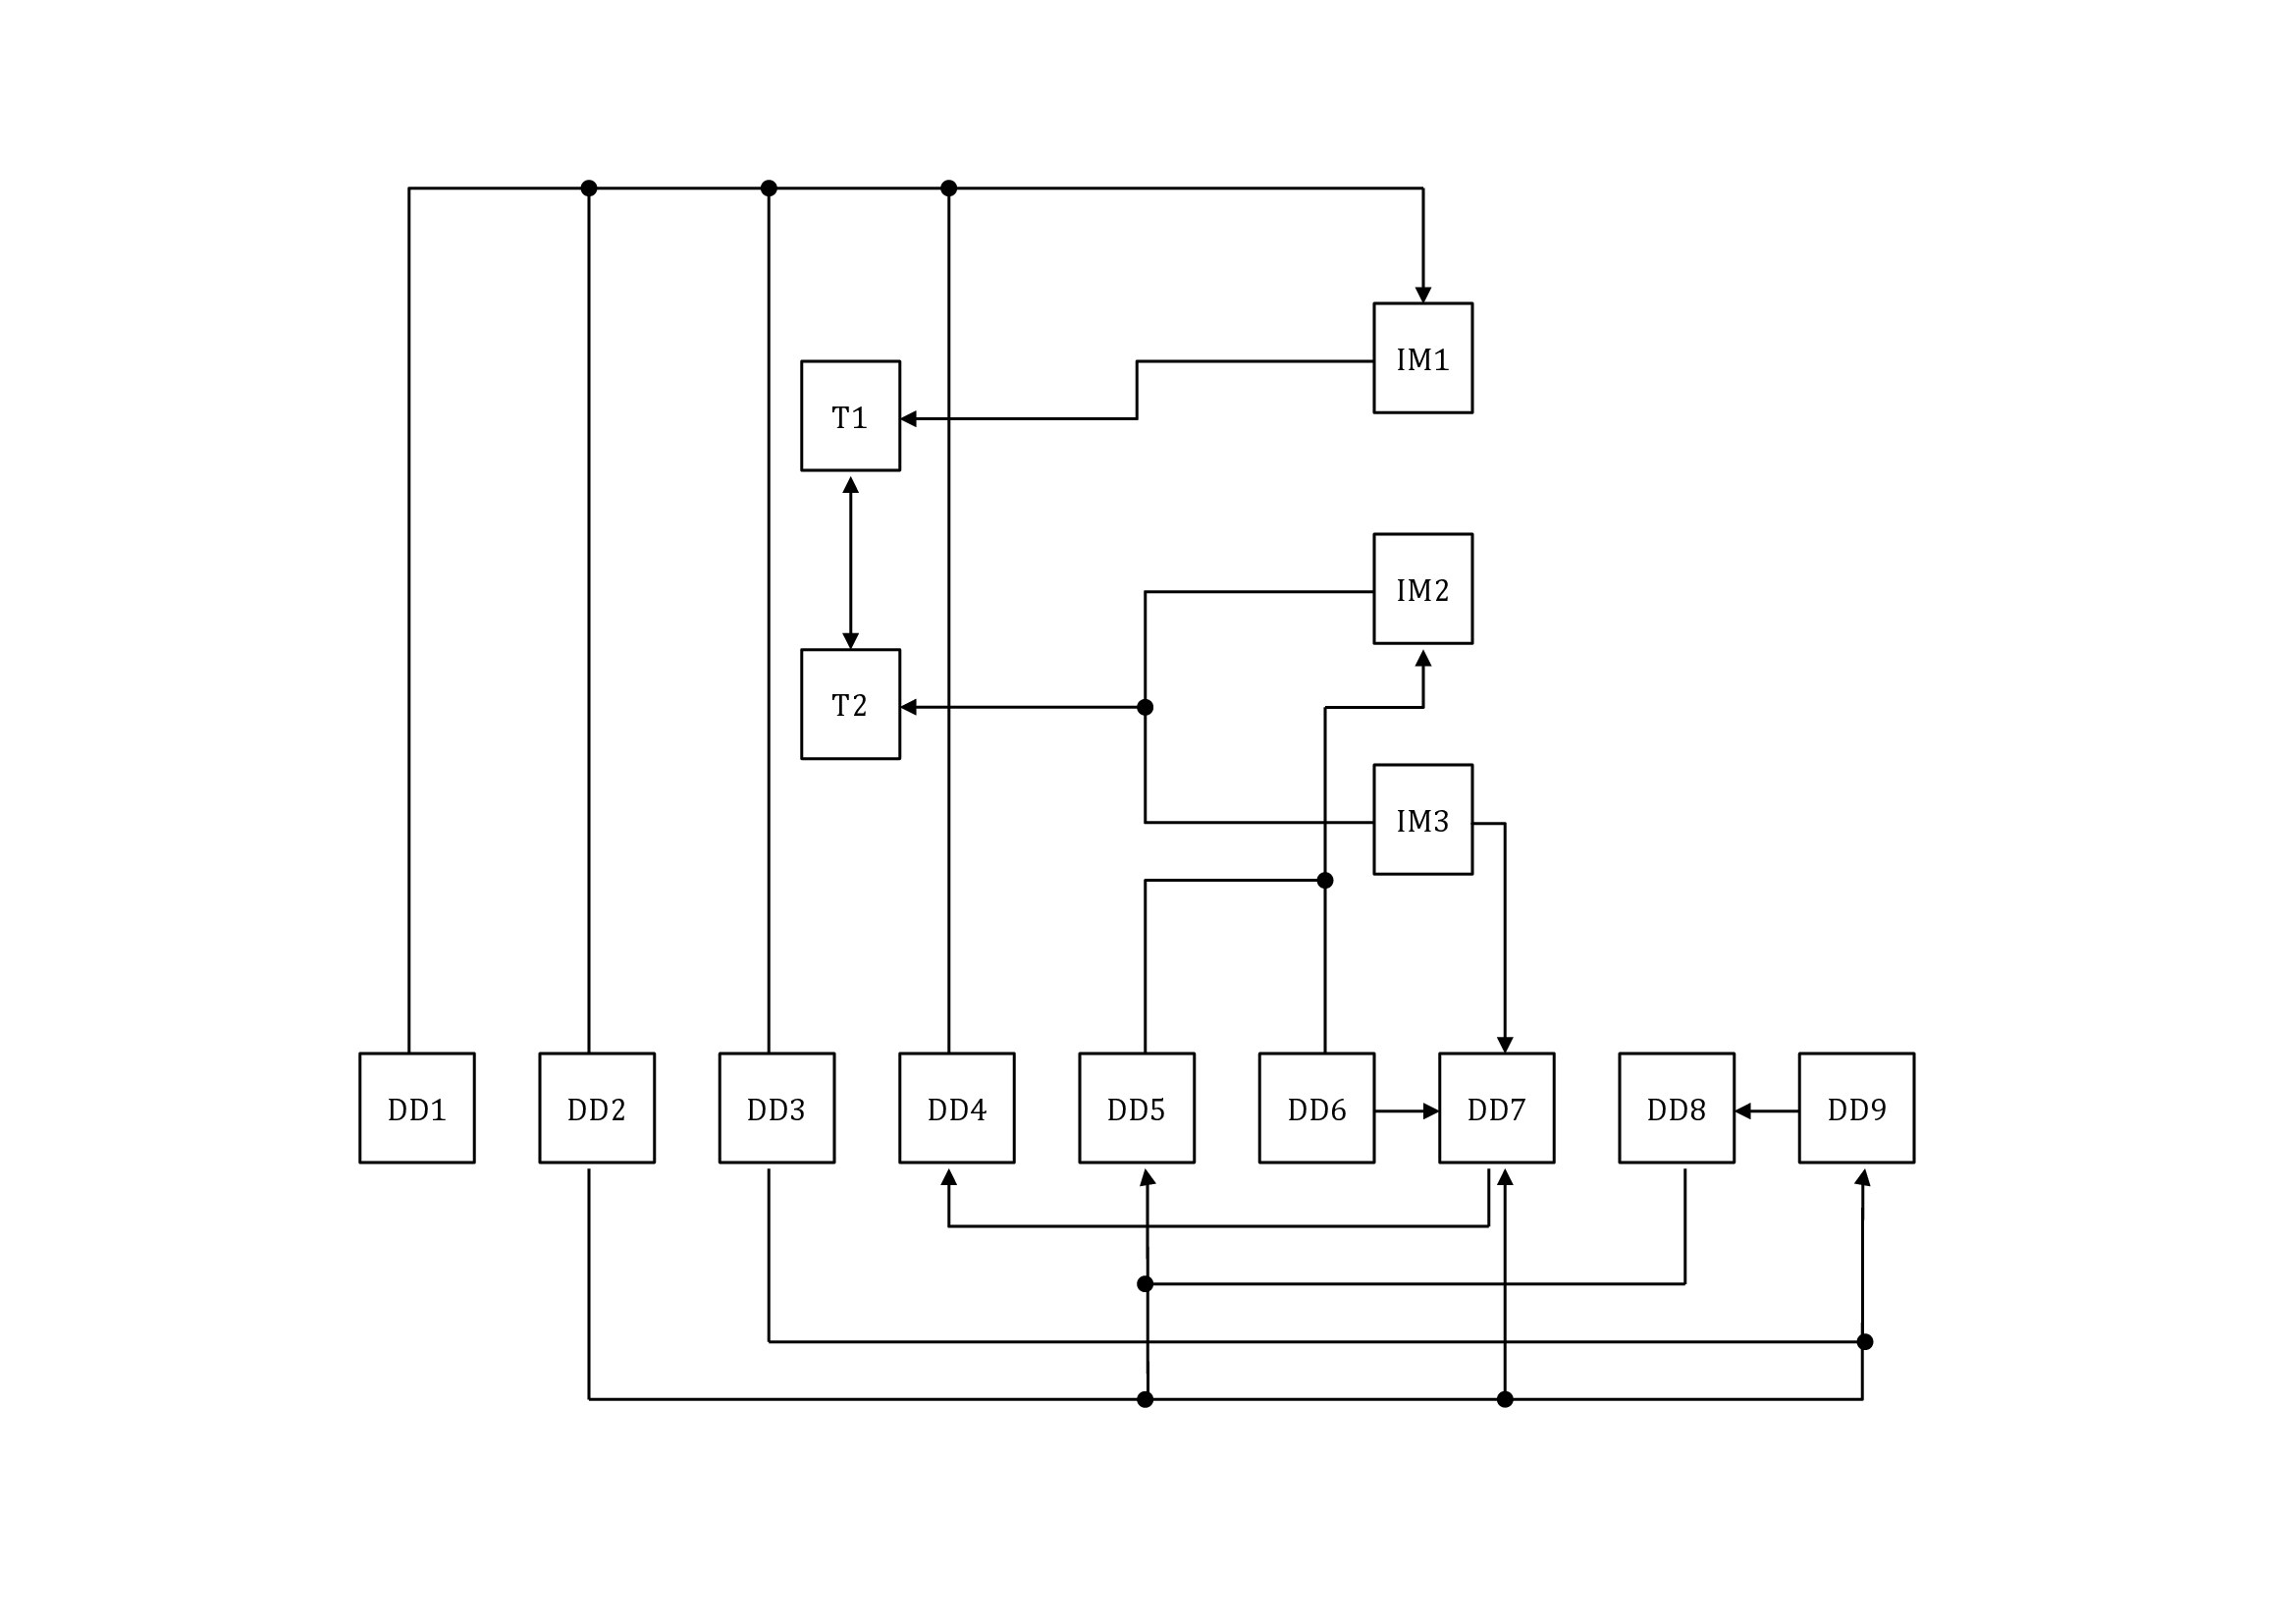
\includegraphics[width=\textwidth]{../../../datafiles/GlassBR/Trace.png}
\caption{Figure 2: Traceability Matrix Showing the Connections Between Items of Different Sections}
\label{Figure:TraceyItemSecs}
\end{center}
\end{figure}
\begin{figure}
\begin{center}
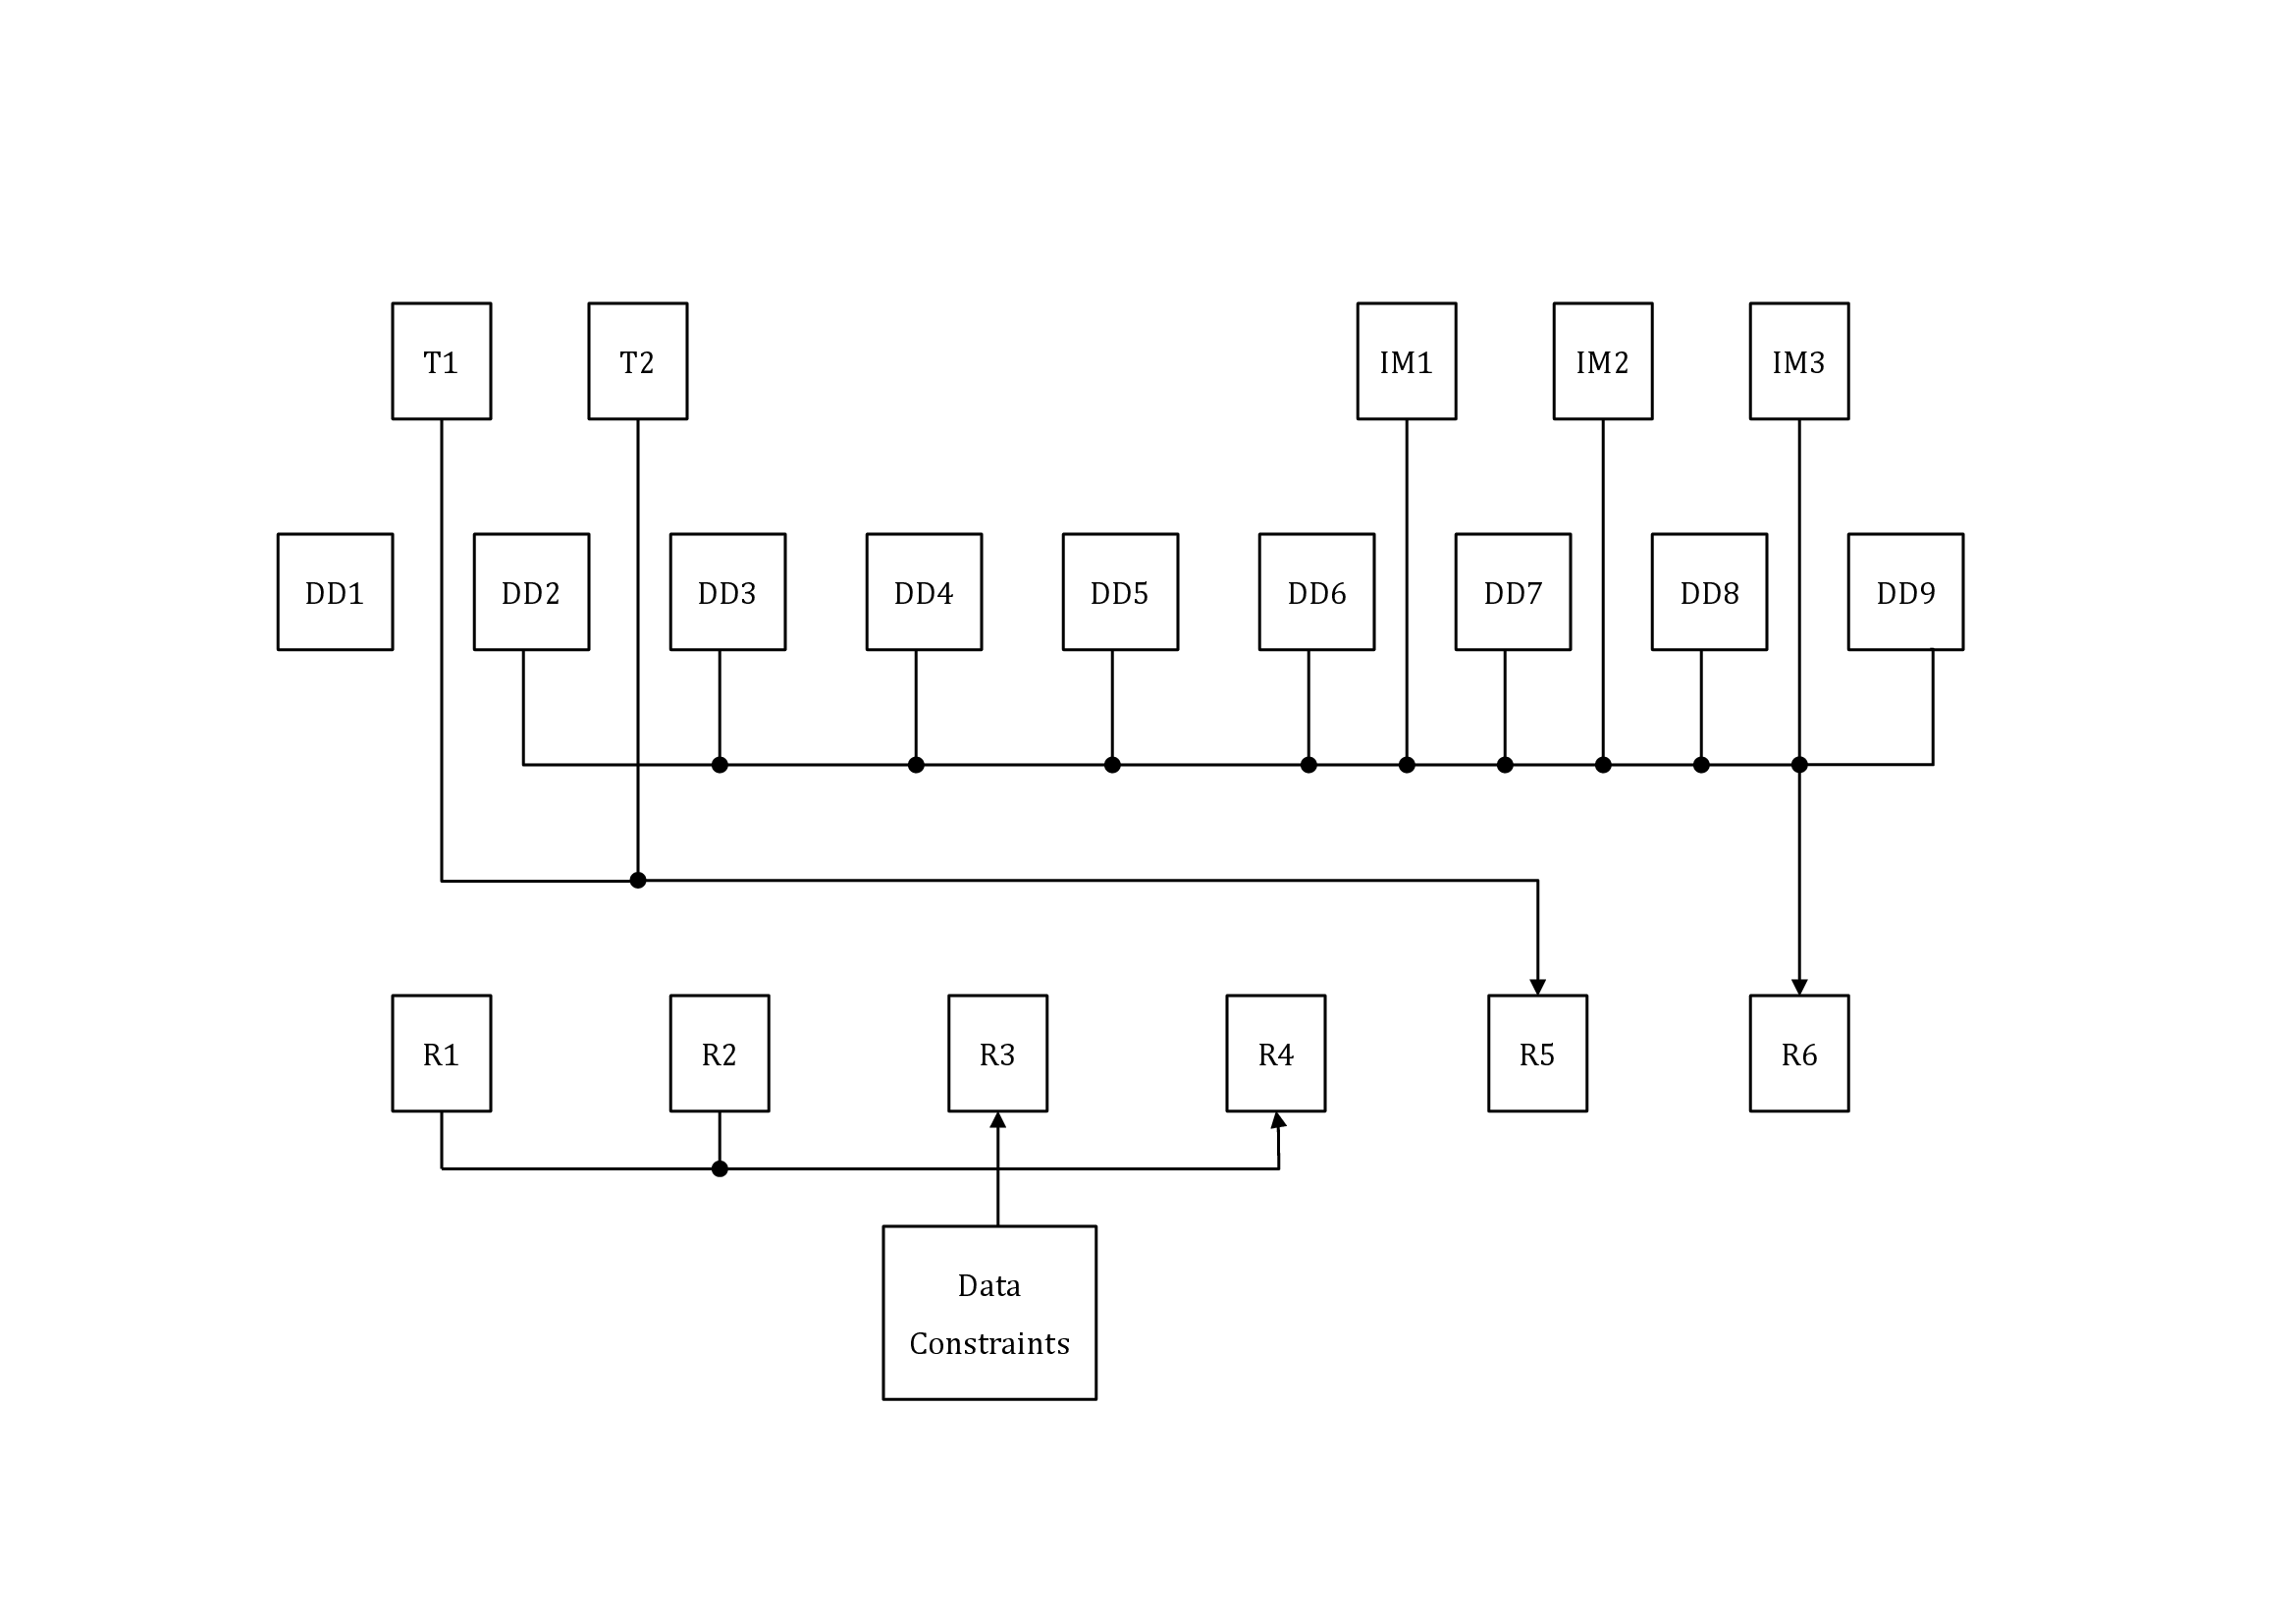
\includegraphics[width=\textwidth]{../../../datafiles/GlassBR/RTrace.png}
\caption{Figure 3: Traceability Matrix Showing the Connections Between Requirements and Other Items}
\label{Figure:TraceyReqsItems}
\end{center}
\end{figure}
\begin{figure}
\begin{center}
\includegraphics[width=\textwidth]{../../../datafiles/GlassBR/ATrace.png}
\caption{Figure 4: Traceability Matrix Showing the Connections Between Assumptions and Other Items}
\label{Figure:TraceyAssumpsOthers}
\end{center}
\end{figure}
\section{Values of Auxiliary Constants}
\label{Sec:AuxConstants}
This section contains the standard values that are used for calculations in GlassBR.
\begin{longtabu}{l X[l] l l}
\toprule
Symbol & Description & Value & Unit
\\
\midrule
${AR_{max}}$ & maximum aspect ratio & $5.0$ & --
\\
${d_{max}}$ & maximum value for one of the dimensions of the glass plate & $5.0$ & m
\\
${d_{min}}$ & minimum value for one of the dimensions of the glass plate & $0.1$ & m
\\
$E$ & modulus of elasticity of glass & $7.17 10^{7}$ & Pa
\\
$k$ & surface flaw parameter & $2.86 10^{-53}$ & $\frac{\text{m}^{12}}{\text{N}^{7}}$
\\
$LSF$ & load share factor & $1$ & --
\\
$m$ & surface flaw parameter & $7$ & $\frac{\text{m}^{12}}{\text{N}^{7}}$
\\
${SD_{max}}$ & maximum stand off distance permissible for input & $130.0$ & m
\\
${SD_{min}}$ & minimum stand off distance permissible for input & $6.0$ & m
\\
${t_{d}}$ & duration of load & $3$ & s
\\
${w_{max}}$ & maximum permissible input charge weight & $910.0$ & kg
\\
${w_{min}}$ & minimum permissible input charge weight & $4.5$ & kg
\\
\bottomrule
\caption{Auxiliary Constants}
\label{Table:TAuxConsts}
\end{longtabu}
\section{References}
\label{Sec:References}
\begin{filecontents*}{bibfile.bib}
@misc{astm2009,
author={ASTM},
title={Standard Practice for Determining Load Resistance of Glass in Buildings},
publisher={ASTM International},
booktitle={Standard E1300-09a},
year={2009},
howpublished={\url{www.astm.org}}}

@misc{astm2012,
author={ASTM},
title={Standard Specification for Heat-Strengthened and Fully Tempered Flat Glass},
publisher={ASTM International},
address={West Conshohocken, PA},
year={2012},
howpublished={\url{https://doi.org/10.1520/C1048-12E01}}}

@misc{astm2016,
author={ASTM},
title={Standard specification for Flat Glass},
publisher={ASTM International},
address={West Conshohocken, PA},
year={2016},
howpublished={\url{https://doi.org/10.1520/C1036-16}}}

@misc{beasonEtAl1998,
author={Beason, W. Lynn and Kohutek, Terry L. and Bracci, Joseph M.},
title={Basis for ASTME E 1300 Annealed Glass Thickness Selection Charts},
booktitle={ASCE Library},
month={feb},
year={1998},
howpublished={\url{doi.org/10.1061/(ASCE)0733-9445(1998)124:2(215)}}}

@booklet{campidelli,
title={Glass-BR Software for the design and risk assessment of glass facades subjected to blast loading},
author={Campidelli, Manuel}}

@mastersthesis{koothoor2013,
author={Koothoor, Nirmitha},
title={A document drive approach to certifying scientific computing software},
school={McMaster University},
year={2013},
address={Hamilton, ON, Canada}}

@article{parnasClements1986,
author={Parnas, David L. and Clements, P. C.},
title={A rational design process: How and why to fake it},
journal={IEEE Transactions on Software Engineering},
year={1986},
month={feb},
volume={12},
number={2},
pages={"251-257"},
address={Washington, USA}}

@misc{rbrtsn2012,
author={Robertson, James and Robertson, Suzanne},
title={Volere requirements specification template edition 16},
howpublished={\url{https://pdfs.semanticscholar.org/cf57/27a59801086cbd3d14e587e09880561dbe22.pdf}},
year={2012}}

@inproceedings{smithLai2005,
author={Smith, W. Spencer and Lai, Lei},
title={A new requirements template for scientific computing},
booktitle={Proceedings of the First International Workshop on Situational Requirements Engineering Processes - Methods, Techniques and Tools to Support Situation-Specific Requirements Engineering Processes, SREP'05},
year={2005},
editor={Agerfalk, PJ and Kraiem, N. and Ralyte, J.},
address={Paris, France},
pages={"107-121"},
note={In conjunction with 13th IEEE International Requirements Engineering Conference,}}
\end{filecontents*}
\nocite{*}
\bibstyle{ieeetr}
\printbibliography[heading=none]
\section{Appendix}
\label{Sec:Appendix}
This appendix holds the graphs (Figure~\ref{Figure:demandVSsod} and Figure~\ref{Figure:dimlessloadVSaspect}) used for interpolating values needed in the models.
\begin{figure}
\begin{center}
\includegraphics[width=\textwidth]{../../../datafiles/GlassBR/ASTM_F2248-09.png}
\caption{Figure 5: 3 second duration equivalent pressure ($q$) versus Stand off distance (SD) versus Charge weight ($w$)}
\label{Figure:demandVSsod}
\end{center}
\end{figure}
\begin{figure}
\begin{center}
\includegraphics[width=\textwidth]{../../../datafiles/GlassBR/ASTM_F2248-09_BeasonEtAl.png}
\caption{Figure 6: Non dimensional lateral load ($\hat{q}$) versus Aspect Ratio (AR) versus Stress distribution factor (Function) ($J$)}
\label{Figure:dimlessloadVSaspect}
\end{center}
\end{figure}
\end{document}
